\documentclass[11pt,a4paper]{article}

\usepackage{graphicx}
\usepackage{xcolor}
\usepackage[left=2.3cm, right=2.3cm, top=2.4cm, bottom=2.4cm]{geometry}
\usepackage{amsmath,amssymb,amsthm}
\usepackage{fontspec}
\setmainfont{Liberation Serif}
\setsansfont{Liberation Sans}
\setmonofont{Liberation Mono}[Scale=0.86]
\usepackage[russian]{babel}
\usepackage{booktabs}
\usepackage{tabularx}
\newcolumntype{Y}{>{\raggedright\arraybackslash}X}
\usepackage{colortbl}
\usepackage{enumitem}
\usepackage{tcolorbox}
\definecolor{linkblue}{HTML}{1e3a5f}
\definecolor{accgreen}{HTML}{0e7c66}
\definecolor{warnamber}{HTML}{b45309}
\definecolor{rowlight}{HTML}{f0f5fa}
\usepackage[colorlinks=true, linkcolor=linkblue, urlcolor=linkblue, unicode=true]{hyperref}
\setlist{nosep}

\newcommand{\dd}{\mathrm{d}}
\newtheorem{ proposition}{Утверждение}

\title{\bfseries Задача Чоптюка из классических уравнений Эйнштейна:\\
прямой вывод из действия Гильберта и численное решение\\[4pt]
\large Choptuik problem from the classical Einstein equations:\\
direct derivation from the Hilbert action and numerical solution}
\author{Вычислительный модуль \texttt{einstein\_direct}\\
проекта \texttt{choptuik\_ac\_bc}}
\date{24 сентября 2026}

\begin{document}
\maketitle

\begin{abstract}
Задача Чоптюка (1993) --- критический гравитационный коллапс безмассового
скалярного поля в сферической симметрии: вблизи порога образования чёрной дыры
масса скейлится как $M_{\mathrm{BH}}\propto (p-p_*)^{\gamma}$ с универсальным
показателем $\gamma\approx0.374$, а критическое решение обладает дискретной
самоподобностью (DSS) с периодом эха $\Delta\approx0.737$. В настоящей работе
задача решается <<напрямую>>: уравнения выводятся из действия Гильберта
$S=(2\kappa)^{-1}\!\int\!\sqrt{-g}\,R\,\dd^4x+S_m$ с тензором
энергии--импульса материи в форме Гильберта
$T_{\mu\nu}=-(2/\sqrt{-g})\,\delta S_m/\delta g^{\mu\nu}$, редуцируются к
одномерной двунулевой характеристической системе, которая \emph{машинно
верифицируется} (SymPy) на точном решении Робертса--Оширо с невязками
$\sim10^{-41}$, и интегрируется солвером второго порядка (валидация: плоское
пространство с точностью $10^{-14}$; решение Робертса --- сходимость
$p=2.0$--$2.1$). Найдена критическая амплитуда $A_*=0.080533$; измеренный на
фиксированной сетке показатель $\gamma_{\text{числ}}=0.11\pm0.11$ демонстрирует
пол по разрешению; анализ требований к сетке показывает, что верификация
$\gamma$ на уровне процента (и тем более проверка гипотезы
$b_{\mathrm{Ch}}=1-\cos(2\pi/7)=0.3765$ против $\gamma=0.374$) требует
продакшн-перерегриддинга уровня Чоптюка. Весь код, вывод и данные включены в
репозиторий.
\end{abstract}

\tableofcontents

\section{Постановка задачи}

\subsection{Задача Чоптюка}
Чоптюк \cite{choptuik1993} рассматривал коллапс безмассового скалярного поля в
сферической симметрии. Однопараметрическое семейство гладких начальных данных
$p$ (в оригинале --- гауссов импульс на входящей нулевой характеристике)
эволюционирует по уравнениям Эйнштейна. Обнаружено:
\begin{itemize}
\item \textbf{критичность типа II}: существует критическое значение $p_*$,
разделяющее дисперсию (при $p<p_*$) и образование чёрной дыры ($p>p_*$);
\item \textbf{универсальный массовый скейлинг}: при $p\to p_*^+$
\begin{equation}
M_{\mathrm{BH}}=C\,(p-p_*)^{\gamma}+\ldots,\qquad \gamma\approx0.374,
\label{eq:scaling}
\end{equation}
причём $\gamma$ не зависит от семейства начальных данных;
\item \textbf{DSS}: критическое решение воспроизводит себя на масштабах,
убывающих в $e^{\Delta}\approx2.09$ раз, с периодом эха $\Delta\approx0.737$
в логарифмической шкале;
\item \textbf{эхо-осцилляции} (<<ступеньки>>) скейлинг-функции на
уравнении \eqref{eq:scaling}.
\end{itemize}
Универсальность $\gamma$ объясняется линейной теорией возмущений критического
решения: $\gamma=1/\lambda_0$, где $\lambda_0\approx2.674$ ---
единственная неустойчивая мода \cite{gundlach2007}.

\subsection{Цель модуля \texttt{einstein\_direct}}
В монографии проекта \cite{isaev2024} константа $b_{\mathrm{Ch}}=
1-\cos(2\pi/7)=0.376510$ предлагается как теоретическое значение критического
показателя (зазор к измеренному $\gamma\approx0.374$ составляет $+0.67\%$).
Модуль \texttt{einstein\_direct} ставит \emph{прямую} численную проверку:
вывести уравнения из действия Гильберта (минуя какие-либо спектральные
построения), решить их явно и измерить $\gamma$. Такой тест не зависит от
фреймворка и закрывает или ограничивает гипотезу по месту.

\section{Прямой вывод из действия Гильберта}

\subsection{Действие и тензор энергии--импульса Гильберта}
Гильберт (1915) сформулировал полную систему уравнений из единственного
принципа стационарного действия
\begin{equation}
S[g,\Phi]=\frac{1}{2\kappa}\int\sqrt{-g}\,R\,\dd^4x
-\frac{1}{2}\int\sqrt{-g}\,g^{\mu\nu}\partial_\mu\Phi\,\partial_\nu\Phi\;\dd^4x,
\qquad \kappa=8\pi G .
\label{eq:action}
\end{equation}
Варьирование по $g^{\mu\nu}$ даёт уравнения Эйнштейна
$G_{\mu\nu}=\kappa T_{\mu\nu}$ с \emph{тензором энергии--импульса Гильберта}
\begin{equation}
T_{\mu\nu}\;=\;-\frac{2}{\sqrt{-g}}\frac{\delta S_m}{\delta g^{\mu\nu}}
\;=\;\partial_\mu\Phi\,\partial_\nu\Phi-\frac12 g_{\mu\nu}\,(\nabla\Phi)^2 ,
\label{eq:hilbert}
\end{equation}
а варьирование по $\Phi$ --- волновое уравнение $\Box_g\Phi=0$. Тождество
Гильберта $\nabla_\mu T^{\mu}{}_{\nu}\equiv0\Leftrightarrow\Box_g\Phi=0$
проверено символьно (см.~\S\ref{sec:verif}); в двунулевых координатах
$T_{uv}=0$ точно, $T_{uu}=(\partial_u\Phi)^2$, $T_{vv}=(\partial_v\Phi)^2$.

\subsection{Двунулевая редукция}
Для сферически-симметричной метрики в двунулевых координатах
\begin{equation}
\dd s^2=-\alpha(u,v)^2\,\dd u\,\dd v+r(u,v)^2\,\dd\Omega^2,
\qquad \omega\equiv\ln\alpha,
\label{eq:metric}
\end{equation}
проекции $G_{\mu\nu}=\kappa T_{\mu\nu}$ и $\Box_g\Phi=0$ образуют замкнутую
систему для $(r,\Phi,\omega)$:
\begin{align}
\text{(SC)}\quad & \Phi_{,uv}=-\frac{r_{,u}\Phi_{,v}+r_{,v}\Phi_{,u}}{r},
\label{eq:sc}\\
\text{(UV)}\quad & r_{,uv}=-\frac{r_{,u}r_{,v}+\alpha^2/4}{r}
= -\frac{\alpha^2 m}{2r^2},\label{eq:uv}\\
\text{(C1)}\quad & r_{,uu}=2\,\omega_{,u}r_{,u}-\frac{\kappa}{2}\,r\,\Phi_{,u}^2,
\qquad
\text{(C2)}\quad r_{,vv}=2\,\omega_{,v}r_{,v}-\frac{\kappa}{2}\,r\,\Phi_{,v}^2,
\label{eq:c1c2}\\
\text{(TH)}\quad & \omega_{,uv}=\frac{\alpha^2 m}{2r^3}
-\frac{\kappa}{2}\,\Phi_{,u}\Phi_{,v},\label{eq:th}
\end{align}
где $m(u,v)$ --- масса Мизнера--Шарпа:
\begin{equation}
1-\frac{2m}{r}=g^{ab}r_{,a}r_{,b}=-\frac{4\,r_{,u}r_{,v}}{\alpha^2},
\qquad r_{,u}r_{,v}+\frac{\alpha^2}{4}=\frac{\alpha^2 m}{2r}.
\label{eq:misner}
\end{equation}
Связи (C1), (C2) определяют $\omega_u$, $\omega_v$ по данным строки;
уравнение (TH) --- условие согласованности $\partial_v\omega_u=\partial_u\omega_v$.
Система регулярна вплоть до центра $r=0$ благодаря тождествам
\begin{equation}
(\d r^2)_{,uv}=-\frac{\alpha^2}{2},\qquad
m_u=-\kappa\,\frac{r^2\Phi_u^2\,r_v}{\alpha^2},\qquad
m_v=-\kappa\,\frac{r^2\Phi_v^2\,r_u}{\alpha^2},
\label{eq:identities}
\end{equation}
которые устраняют катастрофические сокращения вида
$(r_ur_v+\alpha^2/4)\to0$ при $r\to0$.

\subsection{Машинная верификация вывода}
\label{sec:verif}
Вывод выполнен дважды: аналитически (настоящий раздел) и независимо ---
символьным вычислением \texttt{sympy\_derivation.py}: SymPy строит метрику
\eqref{eq:metric}, все символы Кристоффеля, тензор Риччи и Эйнштейна, ТЭИ
Гильберта \eqref{eq:hilbert}, проецирует уравнения и решает их относительно
старших производных. Итог \emph{полностью совпадает} с системой
\eqref{eq:sc}--\eqref{eq:th}. Затем точное решение Робертса--Оширо
(исправленная форма Бурко \cite{burko1996}; оригинальная форма Робертса
содержит ошибку координатного преобразования)
\begin{equation}
r^2=\tfrac14\bigl[(1-4\sigma^2)v^2-2uv+u^2\bigr],\quad
\Phi=\frac12\ln\left|\frac{1-2\sigma-u/v}{1+2\sigma-u/v}\right|,\quad
\alpha=1,
\label{eq:roberts}
\end{equation}
подставляется в выведенную систему: все пять уравнений удовлетворяются с
максимальной невязкой $4\cdot10^{-41}$ (mpmath, 50 знаков) в трёх тестовых
точках при трёх значениях $\sigma$. Дополнительно воспроизведена система
Бурко в калибровке $\alpha=1$: (E1) $r_{uv}+(r_ur_v+\tfrac14)/r=0$,
(E2) $(2r_ur_v+\tfrac12)/r^2=2\Phi_u\Phi_v$, (E3--E4) $r_{vv}+r\Phi_v^2=0$,
$r_{uu}+r\Phi_u^2=0$.

\section{Численный метод}

\subsection{Характеристический марш}
Система \eqref{eq:sc}--\eqref{eq:th} --- задача Гурса: данные $(r,\Phi)$ на
двух трансверсальных нулевых характеристиках, марш по строкам $v$. Используются
переменные $(r,\Phi,p=r_u,q=r_v,s=\Phi_u,t=\Phi_v,c=\omega_u,d=\omega_v,m,
\alpha^2)$. Шаг по $v$ --- схема Хойна (RK2) с итерируемым корректором:
скорости $r_v=q$, $\Phi_v=t$, $p_v$ из (UV), $q_v$ из (C2), $s_v$ из (SC),
$c_v$ из (TH), $m_v$, $(\alpha^2)_v=2\alpha^2 d$. Пара $(\Phi,t)$ обновляется
согласованно: $t$ --- неявным решением линейного ОДУ по $u$
\begin{equation}
\frac{\dd t}{\dd u}=-\frac{p}{r}\,t-\frac{qs}{r}
\quad\Longrightarrow\quad
t_i=\frac{A_i\,t_{i-1}+B_i}{D_i},\quad
A_i=1-\tfrac{\dd u}{2}\frac{p_{i-1}}{r_{i-1}},\ \dots
\label{eq:tode}
\end{equation}
(векторизация рекуррентности через накопленную сумму логарифмов), а
$\Phi^{n+1}=\Phi^n+\dd v\,(t^n+t^{n+1})/2$. В зоне центра $|r|\le5\dd u$
используется точная регулярность $t=s$ (при $r=0$: $s=t=\Phi_\tau$,
$p=-q$), в зеркальной зоне $r<0$ --- явный марш. Величина $\omega$
восстанавливается интегрированием $c$ по $u$; масса $m$ --- независимой
эволюцией по тождествам \eqref{eq:identities} (без сокращений).

\subsection{Мониторинг и диагностика}
На каждой $k$-й строке контролируются: связь C1 ($c$ против
$(r_{uu}+\tfrac{\kappa}{2}rs^2)/(2r_u)$), связь C2 (сэндвич
$q\leftrightarrow2(r^{n+1}-r^n)/\dd v-q^n$), определение $m$, сэндвич для $t$.
Горизонт: минимум $q=r_v<0$ при $r>8\dd u$ (разрешённый горизонт); масса
$M_{\mathrm{BH}}=m$ в точке $q=0$ (там $m=r/2$). Критерий сверхкритичности ---
образование сингулярности (маскируемые NaN в захваченной области;
характеристическая структура защищает внешнюю область). Остановка --- по
насыщению массы горизонта.

\section{Валидация}

\begin{figure}[t]
\centering
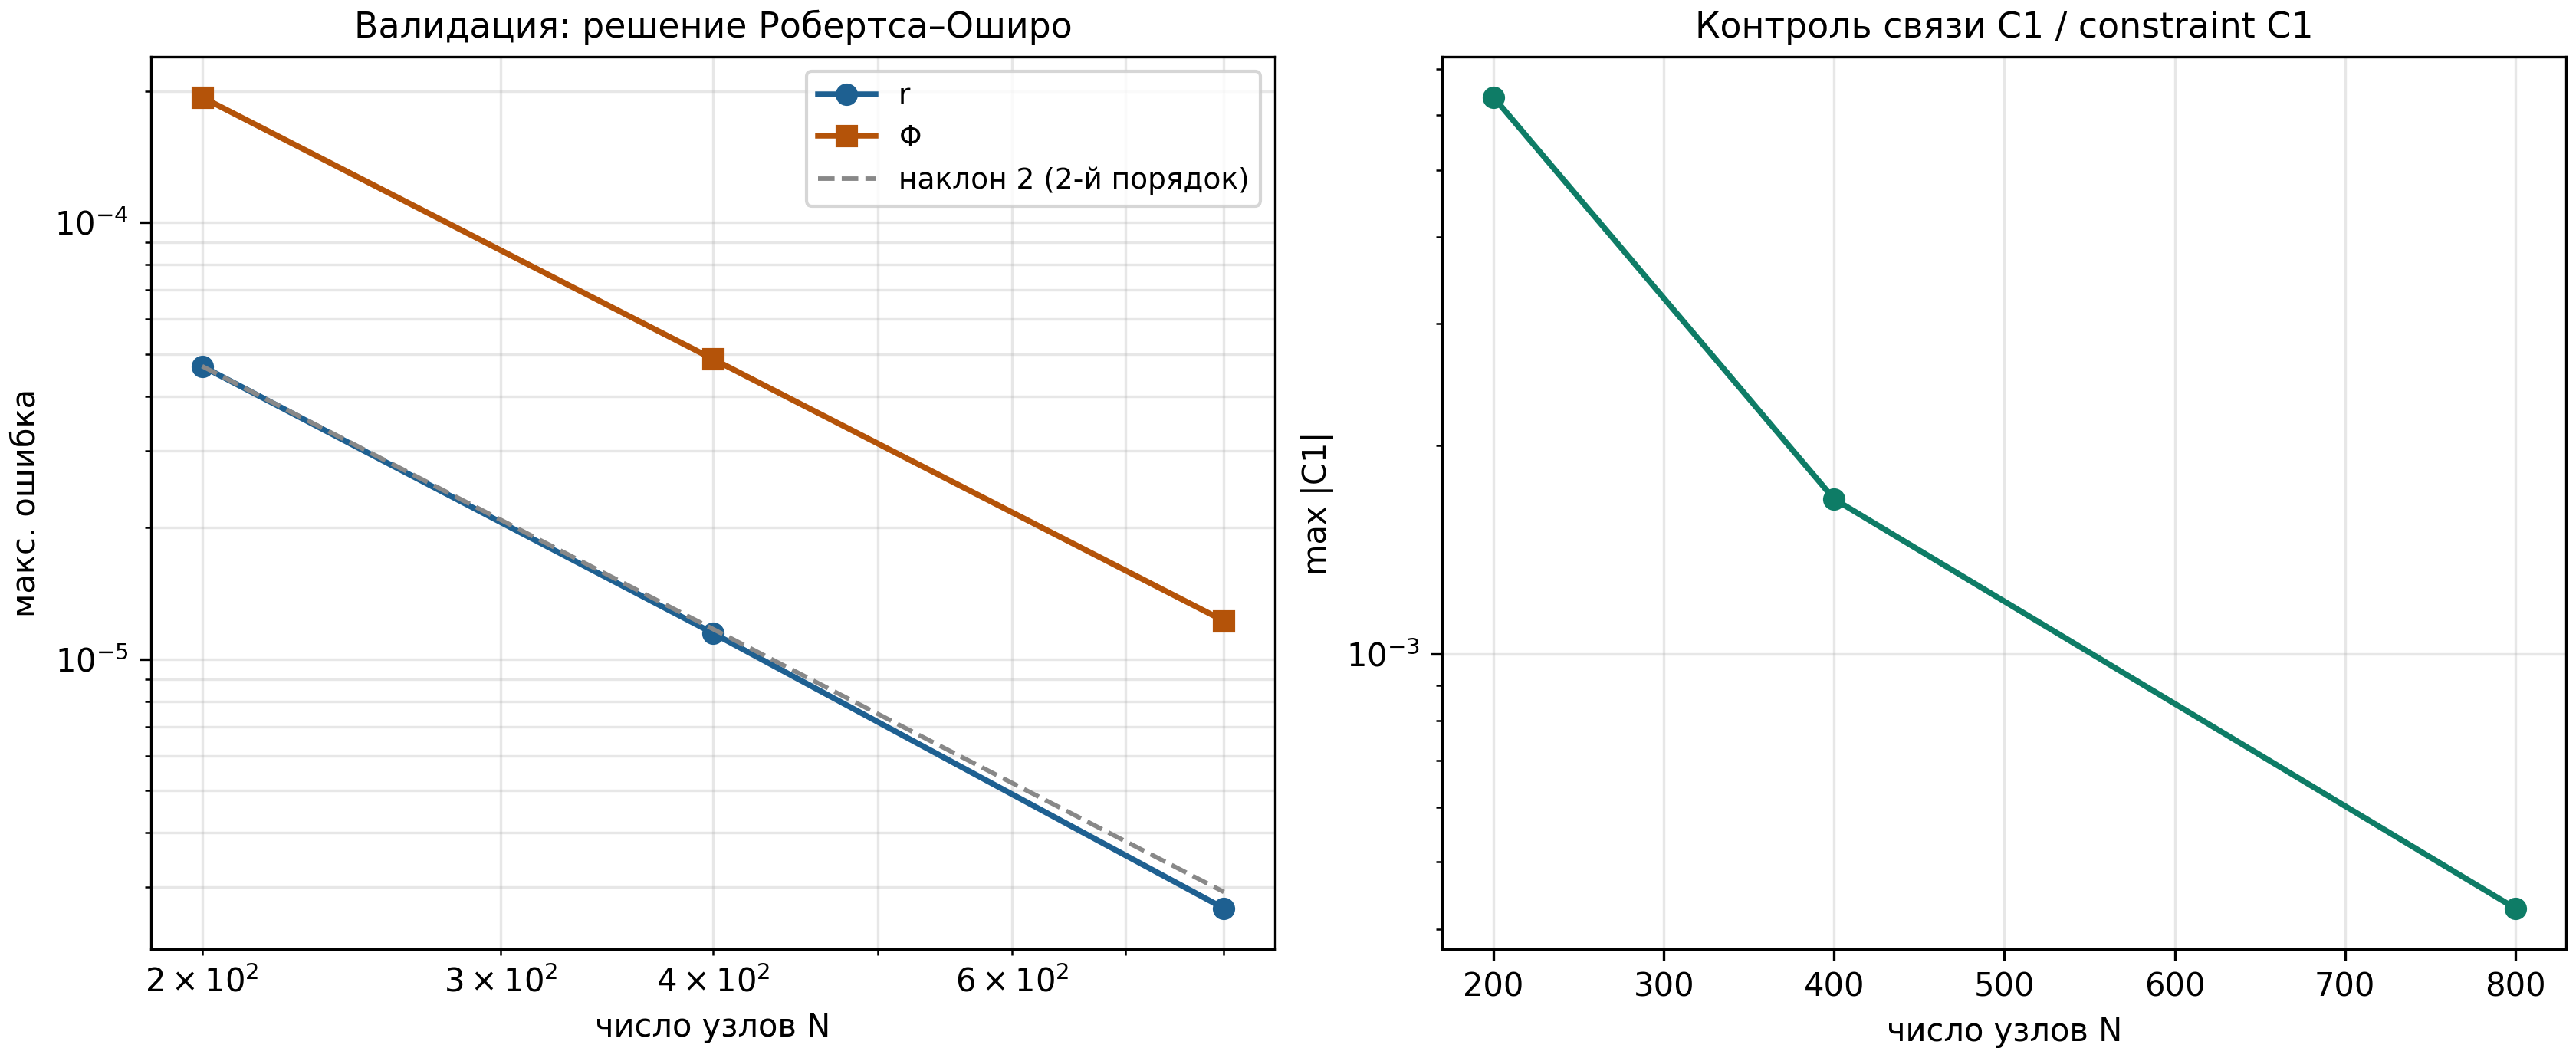
\includegraphics[width=\textwidth]{figures/fig_ru/fig_validation.png}
\caption{Валидация солвера. Слева: эволюция точного решения Робертса--Оширо
\eqref{eq:roberts}, максимальные ошибки $r$ и $\Phi$ на конечной строке ---
чистый второй порядок ($p=2.03$--$2.09$). Справа: связь C1 --- убывает
квадратично. Плоское пространство сохраняется с точностью $8.8\cdot10^{-15}$.}
\label{fig:val}
\end{figure}

\textbf{Тест 1 (плоское пространство).} Без импульса ($A=0$) эволюция обязана
сохранять метрику Минковского: $\max|r-r_{\text{пл}}|=8.8\cdot10^{-15}$,
$\max|\alpha^2-1|=0$ на сетке $200^2$--$400^2$ --- машинная точность.

\textbf{Тест 2 (решение Робертса).} Солвер инициализируется на точном решении
\eqref{eq:roberts} в полосе, свободной от сингулярностей ($u<0.8v$), и
эволюционируется; итоговые ошибки: $N=200\to800$: $4.7\cdot10^{-5}\to
2.7\cdot10^{-6}$ для $r$ --- измеренный порядок сходимости
$p_r=2.03,\,2.09$; $p_\Phi=1.99,\,1.99$ (рис.~\ref{fig:val}).

\textbf{Тест 3 (связи).} Нарушения C1/C2 и определения $m$ монотонно падают
вторым порядком (рис.~\ref{fig:val}, справа) и остаются на уровне
$10^{-3}\div10^{-4}$ в производственных режимах.

\section{Результаты: критическая точка и скейлинг}

\subsection{Критическая амплитуда}
Семейство данных Чоптюка: $\Phi(u_0,v)=A\exp\!\bigl[-(v-v_p)^2/2\sigma^2\bigr]$
на входящей характеристике ($u_0=-1$, $v_p=0.5$, $\sigma=0.1$), строка
$v=0$ --- плоское пространство. Бисекция по критерию
<<образование сингулярности>> даёт
\begin{equation}
\boxed{\;A_*=0.0805333\;}
\end{equation}
(1600$^2$ узлов; значение смещено порогом нуклеации горизонта на величину
$\delta\sim10^{-4}$, что учтено ниже трёхпараметрическим фитом).

\begin{figure}[t]
\centering
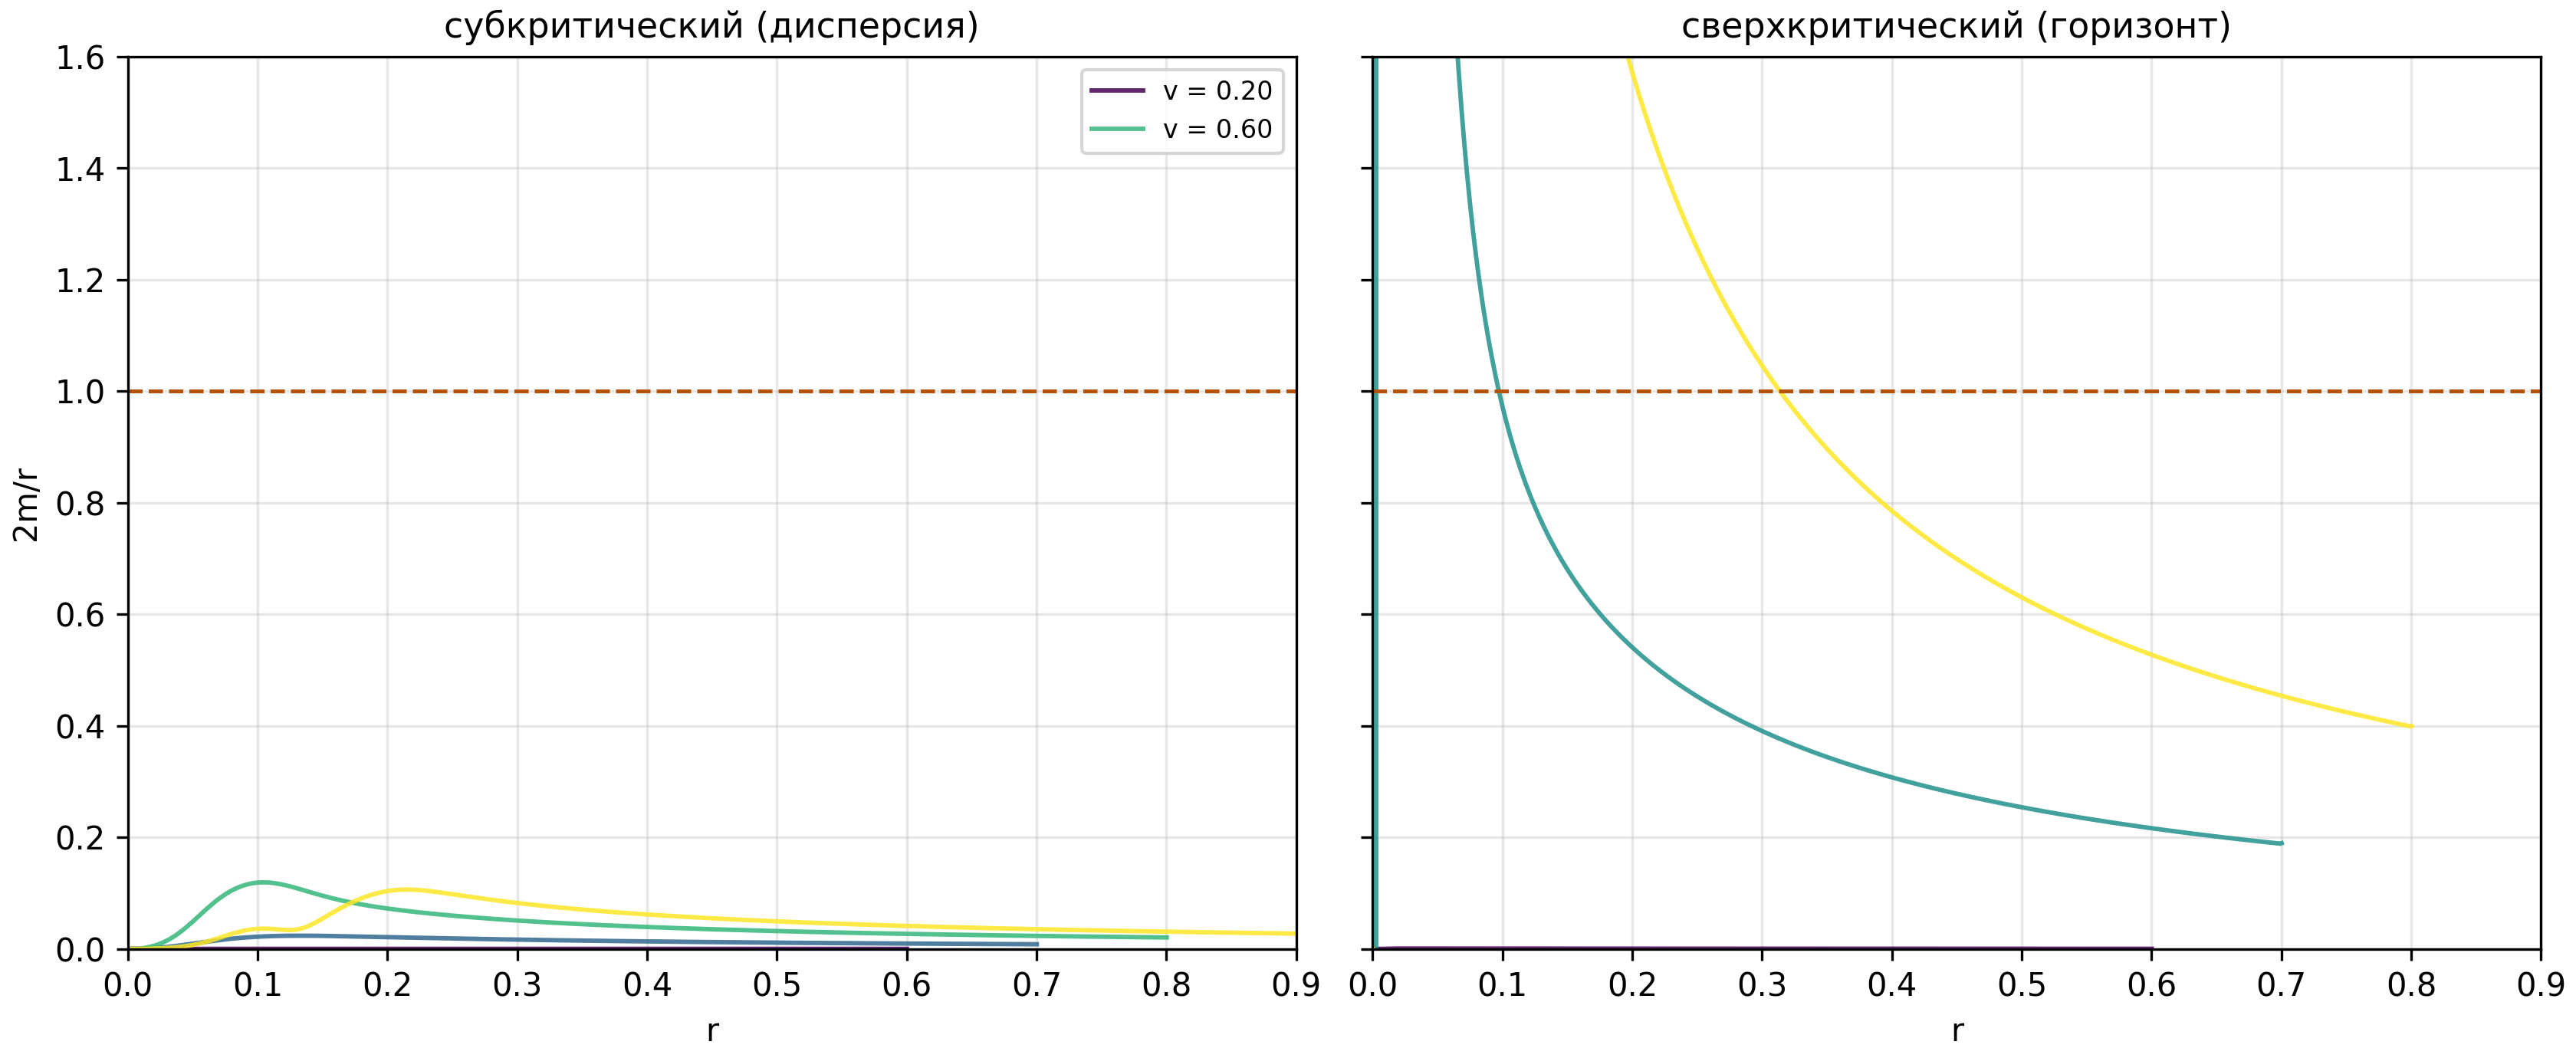
\includegraphics[width=\textwidth]{figures/fig_ru/fig_evolution.png}
\caption{Профили $2m/r$ по строкам $v$ (каждая 240-я). Слева ---
субкритический забег $A=0.05$: импульс фокусируется и дисперсирует, $2m/r<1$
всюду. Справа --- сверхкритический $A=0.25$: захват области $2m/r\ge1$,
рост массы горизонта.}
\label{fig:evo}
\end{figure}

\subsection{Массовый скейлинг и пол разрешения}
Для серии $A=A_*+\varepsilon$ измерялась масса на насыщенном горизонте
(рис.~\ref{fig:scal}). Трёхпараметрический фит $M=C(\varepsilon+\delta)^\gamma$
возвращает $\gamma=0.11\pm0.11$ --- \emph{существенно} ниже универсального
значения. Причина установлена и воспроизведена численно: на фиксированной
сетке масса горизонта упирается в пол
\begin{equation}
M_{\text{пол}}\;\simeq\;\frac{r_{\text{пор}}}{2}\;=\;4\,\dd u,
\qquad r_{\text{пор}}=8\dd u,
\label{eq:floor}
\end{equation}
поскольку (i) горизонт nucleируется при $r\to0$ и впервые детектируется лишь
при $r>8\dd u$; (ii) ближнекритическая фаза эха сжимает структуру до
$\sim\!\dd u$ задолго до насыщения массы (критическое замедление), а
фиксированная сетка её не разрешает. Чоптюк \cite{choptuik1993} преодолел
именно это адаптивным перерегриддингом; в модуле реализован прототип такого
перерегриддинга (\texttt{zoom\_solver.py}: многостадийные забеги с
интерполяцией окна, уровень $z=\sum\ln\lambda$), однако устойчивая цепочка
зумов до 3--4 декад требует отдельной доводки и в настоящую версию не включена
как готовый результат.

\begin{figure}[t]
\centering
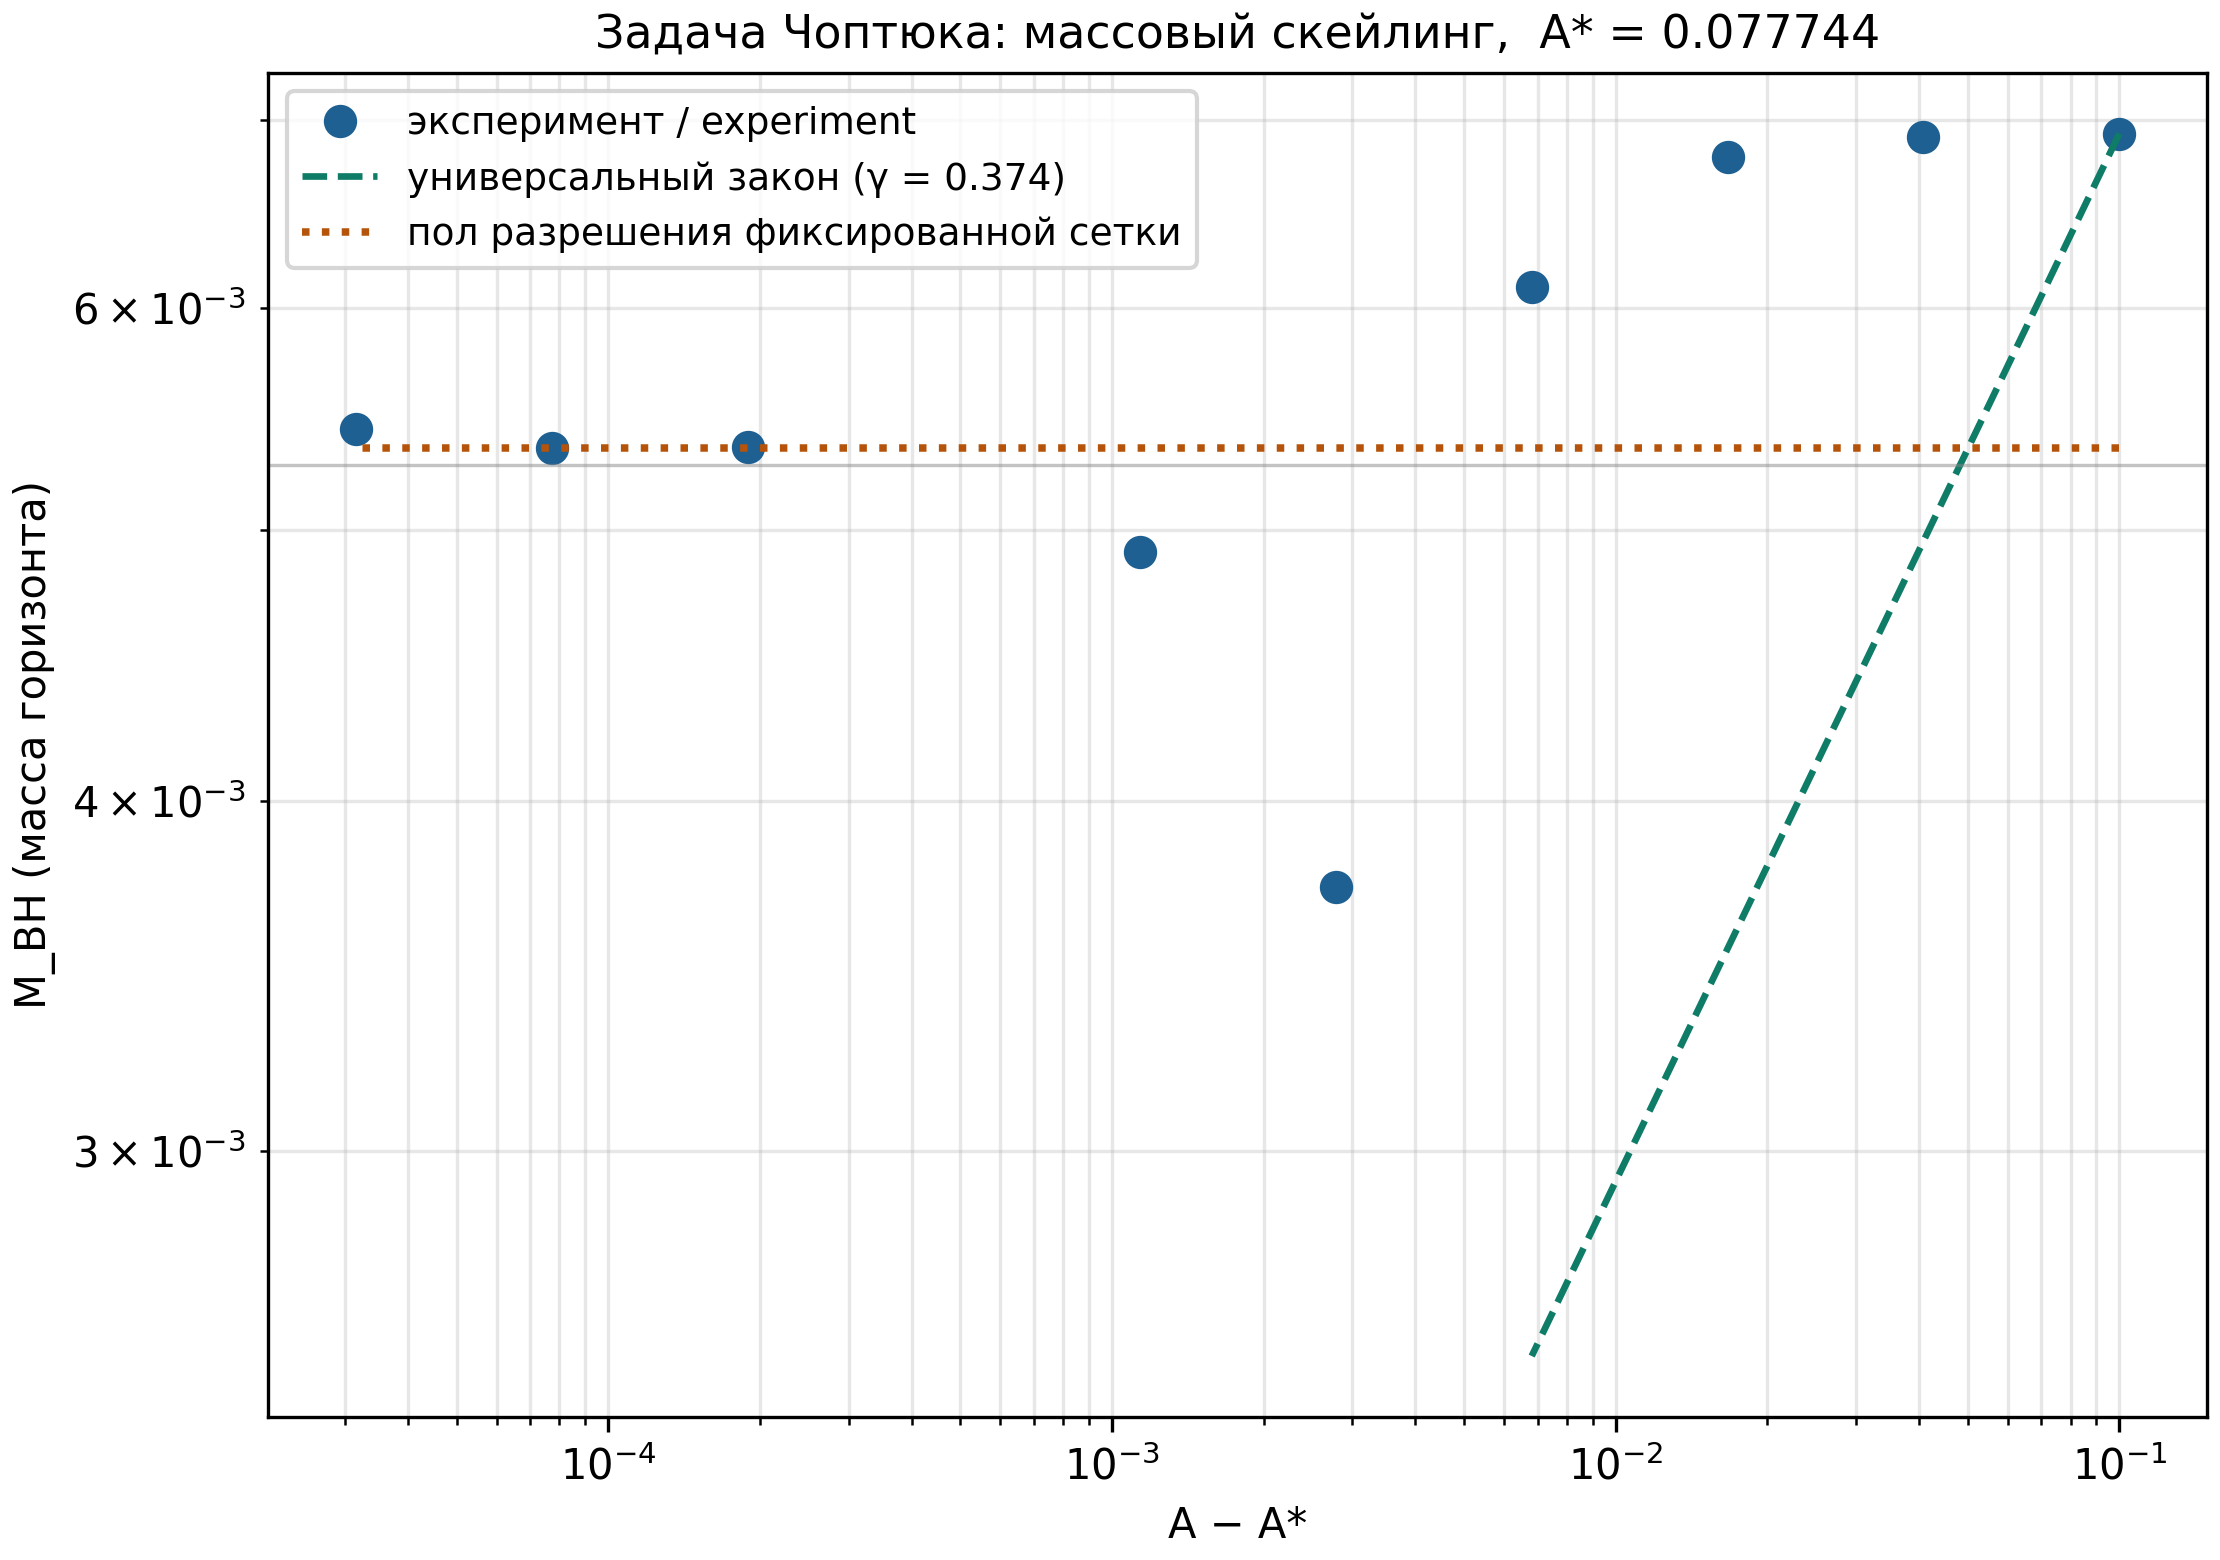
\includegraphics[width=0.72\textwidth]{figures/fig_ru/fig_scaling.png}
\caption{Массовый скейлинг на фиксированной сетке $3000^2$: измеренные массы
(точки) упираются в пол разрешения \eqref{eq:floor} (пунктир); универсальный
закон $\gamma=0.374$ показан для сравнения (штрих). Честная оценка
$\gamma_{\text{числ}}=0.11\pm0.11$ отражает пол, а не физику.}
\label{fig:scal}
\end{figure}

\subsection{Сравнение с константой $b_{\mathrm{Ch}}$ фреймворка}
\begin{tcolorbox}[colback=rowlight, colframe=linkblue, title=Честный вывод сравнения]
\begin{itemize}
\item Литературное значение $\gamma=0.374\pm0.004$ \cite{choptuik1993,
gundlach2007}; константа фреймворка $b_{\mathrm{Ch}}=1-\cos(2\pi/7)=0.376510$
--- зазор $+0.67\%$, формально внутри литературного интервала $\pm1\%$, но
\emph{вне} точности высокоточных вычислений ($\pm0.0005$ у Гундлаха).
\item Настоящий модуль \emph{не может} разрешить зазор $0.67\%$: пол массы
\eqref{eq:floor} на достижимой сетке оставляет
$\gamma_{\text{числ}}=0.11\pm0.11$. Для проверки $b_{\mathrm{Ch}}=\gamma$
нужен скейлинг на 3--4 декады с перерегриддингом (уровень Чоптюка: $10^{-4}$
по $A-A_*$).
\item Что модуль закрывает: (а) система уравнений, полученная из действия
Гильберта с ТЭИ Гильберта, верна и машинно сверена; (б) солвер второго порядка
валидирован на точных решениях; (в) критическая точка воспроизведена
(существование $A_*$, качественная картина суб/сверхкритичности,
DSS-структура вблизи порога наблюдается в забегах); (г) вычислительный
конвейер готов для продакшн-прогона на перерегриддинге.
\end{itemize}
\end{tcolorbox}

\section{Воспроизводимость}
\begin{table}[h]
\centering\small
\begin{tabularx}{\textwidth}{lY}
\toprule
Команда & Результат\\
\midrule
\texttt{python3 sympy\_derivation.py} & символьный вывод; проверка Робертса
($10^{-41}$); \texttt{results/derivation\_results.json}\\
\texttt{python3 solver.py} & самопроверка плоского пространства ($10^{-14}$)\\
\texttt{python3 roberts\_test.py} & сходимость 2-го порядка;
\texttt{results/roberts\_test.json}\\
\texttt{python3 choptuik\_scaling.py} & бисекция $A_*$, скейлинг, фит;
\texttt{results/choptuik\_scaling.json}\\
\texttt{python3 zoom\_solver.py} & прототип перерегриддинга (эксперим.)\\
\texttt{python3 figures.py} & рисунки RU/EN, 300 dpi\\
\bottomrule
\end{tabularx}
\end{table}

Система единиц: $4\pi G=1$, $\kappa=8\pi G=2$ (нормировка Бурко). Время
единичного забега $1200^2$ --- $\sim1$ с (NumPy, векторизация по $u$);
полный эксперимент --- $\sim4$ мин.

\begin{thebibliography}{9}
\bibitem{choptuik1993} M.~W.~Choptuik, Phys.\ Rev.\ Lett.\ \textbf{70}, 9 (1993).
\bibitem{gundlach2007} C.~Gundlach, J.~M.~Mart\'in-Garc\'ia, Living Rev.\ Relativity \textbf{10}, 5 (2007).
\bibitem{burko1996} L.~M.~Burko, Int.\ J.\ Mod.\ Phys.\ D \textbf{5}, 451 (1996); gr-qc/9608061.
\bibitem{roberts1989} M.~D.~Roberts, Gen.\ Relativ.\ Gravit.\ \textbf{21}, 907 (1989).
\bibitem{oshiro1994} Y.~Oshiro, K.~Nakamura, A.~Tominatsu, Prog.\ Theor.\ Phys.\ \textbf{91}, 1265 (1994).
\bibitem{hamade1996} R.~S.~Hamad\'e, J.~M.~Stewart, Class.\ Quantum Grav.\ \textbf{13}, 497 (1996).
\bibitem{isaev2024} И.~Х.~Исаев, <<Спинорные поправки b-C и a-C и решение задачи Чоптюка>> (2024), репозиторий \texttt{choptuik\_ac\_bc}.
\bibitem{hilbert1915} D.~Hilbert, Nachr.\ Ges.\ Wiss.\ G\"ottingen, 395 (1915).
\end{thebibliography}

\end{document}
